% !TEX encoding = UTF-8
% !TEX TS-program = pdflatex
% !TEX root = ../tesi.tex

%**************************************************************
\chapter{L'applicazione}
\label{cap:applicazione}
%**************************************************************

%\intro{Breve introduzione al capitolo}\\

\section{Introduzione alle grammatiche}
Zucchetti negli ultimi anni ha investito molto nella ricerca di una tecnologia che gli permettesse di interagire con i propri prodotti attraverso comandi vocali ed ora sta realizzando delle regole che permettono la generazione di una \emph{\gls{gramg}} capace di comprendere ed elaborare il linguaggio naturale. \\
Gli assistenti virtuali presenti sul mercato sono basati sul seguente concetto: provare a capire tutto ciò che viene detto dagli utenti anche a costo di commettere degli errori. Questa filosofia è mirata a dare all'utente la sensazione di utilizzare uno strumento in grado di capire e ragionare in qualsiasi momento e condizione ed è già utilizzata in larga scala da grandi aziende quali Google, Amazon e Apple. Tuttavia, per le funzionalità della maggior parte dei prodotti Zucchetti, tale principio non è applicabile. Infatti necessitano che, quando una frase viene riconosciuta e compresa, il margine di errore sia nullo. \\
Un classico esempio è il trasferimento di denaro in cui se la comprensione del comando avviene in modo errato c'è il rischio di causa danni contingenti agli utenti. Dunque Zucchetti ha intrapreso una strada diversa, mirata a alla massima precisione accettando talvolta di non riconoscere i comandi ricevuti. \\
La tecnologia che stanno sviluppando consiste in regole molto semplici ed intuitive da applicare, riassunte in tre azioni principali:
\begin{itemize}
	\item concatenazione di elementi;
	\item scelta tra più elementi;
	\item opzionalità di un elemento.
\end{itemize}
A partire da queste regole viene costruita una \emph{\gls{gramg}} dove ad ogni elemento corrisponde una stringa che rappresenta una qualsiasi parola nel linguaggio naturale. Un esempio semplice ma dimostrativo è illustrato nella seguente immagine.

\begin{figure}[htbp]
	\begin{center}
		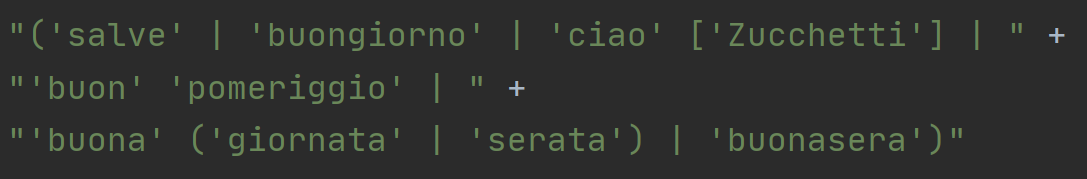
\includegraphics[height=2cm, width=\linewidth]{esempio-grammatica.PNG}
		\caption{Esempio di una grammatica}
	\end{center}
\end{figure}

\vspace{5cm}

Nonostante il loro principio di funzionamento sia relativamente semplice da comprendere, non sono altrettanto facili da interpretare qualora raggiungessero grandi dimensioni e, a maggior ragione, per uno sviluppatore terzo che in futuro le dovrà riutilizzare. Per migliorare questo aspetto l'azienda ha quindi deciso di utilizzare i diagrammi \emph{\gls{rldg}}\glsfirstoccur come strumento di rappresentazione come si può vedere nella figura successiva.

\begin{figure}[htbp]
	\begin{center}
		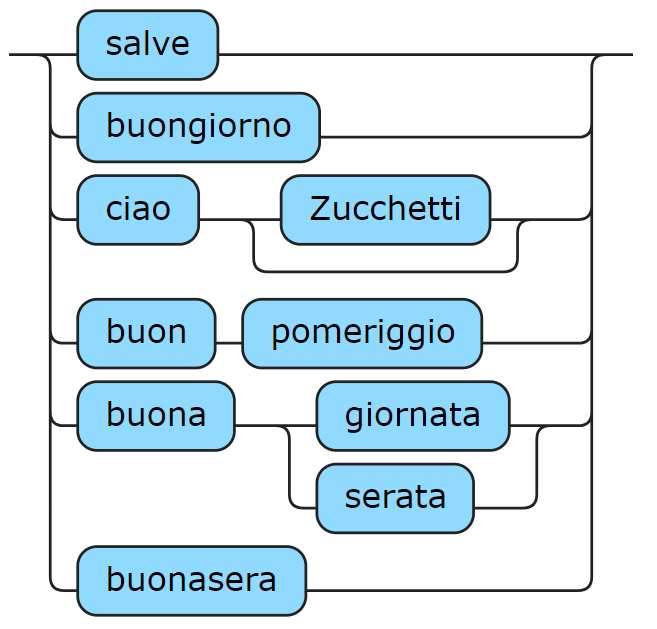
\includegraphics[height=6cm]{esempio-railroad.PNG}
		\caption{Esempio di una grammatica con railroad}
	\end{center}
\end{figure}

Risulta evidente come questa raffigurazione sia molto più efficace e intuitiva. \\
Infine l'applicazione della \emph{\gls{gramg}} sui comandi vocali dell'utente tradotti in stringa avviene attraverso un apposito \emph{\gls{parsg}}\glsfirstoccur sviluppato da Zucchetti che mi è stato consegnato per lo sviluppo del mio progetto.
\section{Analisi dei requisiti}
	\subsection{Descrizione}
	\subsection{Obiettivi}

\section{Progettazione}
	\subsection{Interfaccia vocale}
	\subsection{NLU}
	\subsection{Capacità conversazionale}

\section{Implementazione}

\section{Test}

\section{Sviluppi futuri}
